\chapter{Các công trình liên quan}

\section{Các công trình nghiên cứu liên quan đến Chatbot hỗ trợ thương mại điện tử}
\subsection{Bài báo về Chatbot hỗ trợ y tế tự động}
Đây là bài báo có tên \textit{Automated Medical Chatbot} \cite{automatedmedical}. Trong bài báo này, tác giả đề xuất một hệ thống có khả năng đặt ra nhiều câu hỏi cho người dùng cho đến khi xác định được căn bệnh mà người dùng đang gặp phải. Đây gần như là một hệ thống tư vấn y tế. Hệ thống sẽ thu thập các thông tin từ người dùng như triệu chứng, sau đó đưa ra những căn bệnh mà người dùng có thể mắc phải và hỏi người dùng về cảm giác của họ. Sau khi nhận được nhiều dữ liệu, nó sẽ tìm ra căn bệnh có khả năng xảy ra nhất.

Ngoài ra, họ đặt ra một khái niệm mức ngưỡng giúp phát hiện mức độ của vấn đề. Tuỳ vào mức độ nghiêm trọng của bệnh mà nó sẽ đề xuất các biện pháp khắc phục và thuốc cho người dùng hoặc kết nối người dùng với bác sĩ.

Trong bài báo, tác giả đã sử dụng phương pháp AIML (Artificial Intelligence Mark-up Language) để hiểu được các mẫu (pattern) trong tin nhắn của người dùng thông qua các thẻ (tag) được xác định trước.

Ví dụ, ta có một số các \textit{pattern tag} được xác định trước như ví dụ \ref{exam:pattern}. Khi người dùng nói "I am suffering from headache." (Tôi đang bị đau đầu), hệ thống sẽ ánh xạ tin nhắn của người dùng với các pattern và phát hiện trùng với pattern "I am suffering from *", "headache" (đau đầu) sẽ được thay thế bởi dấu *. Sau đó hệ thống sẽ truy cập vào cơ sở dữ liệu với thông tin đầu tiên là triệu chứng đau đầu và đưa ra hành động tiếp theo.

\renewcommand{\lstlistingname}{Ví dụ}
\begin{lstlisting}[caption={Một số các pattern tag},label={exam:pattern},language=exam_en,firstnumber=1]
<pattern>I am feeling like *</pattern>
<pattern>I am having *</pattern>
<pattern>I am suffering from *</pattern>
\end{lstlisting}

Cùng với một số các thành phần khác thì hệ thống của họ đưa ra có thể tư vấn khách hàng như ví dụ \ref{exam:medicaldialog}. Đầu tiên có thể thực hiện với câu chào hỏi, và hỏi về vấn đề của người dùng. Sau khi nhận được thông tin về triệu chứng là đau đầu, Chatbot sẽ hỏi thêm các thông tin triệu chứng khác để làm rõ căn bệnh. Cuối cùng sau khi lấy đủ thông tin, Chatbot đưa ra kết luận về căn bệnh người dùng mắc phải và cách chữa trị.

\renewcommand{\lstlistingname}{Ví dụ}
\begin{lstlisting}[caption={Một mẫu hội thoại của Chatbot},label={exam:medicaldialog},language=exam_en,firstnumber=1]
User: Hello
Chatbot: Hi there, tell me how can I help you?
User: I am having an Headache
Chatbot: Are you having pain in your eyes?
User: Yes
Chatbot: Do you feel like vomiting?
User: yes I do
Chatbot: I think you are most likely having a migraine attack
Chatbot: Taking "ibuprofen" 2 tablets would reduce pain in you eyes. Also take "aspirin" 20ml to help you tackle vomiting. Do take a nap and dont forget to wash your eyes with luke warm water. Avoid using digital screen until you feel better.
\end{lstlisting}

\subsection{Bài báo về Chatbot hỗ trợ mua sắm trực tuyến}
Đây là bài báo có tên \textit{SuperAgent: A Customer Service Chatbot for E-commerce Websites} \cite{superagent}. Trong bài báo này, họ giới thiệu SuperAgent, một Chatbot dịch vụ khách hàng, sử dụng dữ liệu thương mại điện tử quy mô lớn và công khai. SuperAgent tận dụng dữ liệu từ mô tả sản phẩm trong trang cũng như nội dung do người dùng tạo từ các trang web thương mại điện tử. Ngoài ra, SuperAgent sinh câu phản hồi dựa trên bốn mô hình chạy song song, bao gồm các bộ câu hỏi và trả lời (QA) thực tế, bộ tìm kiếm QA thường gặp, bộ QA văn bản định hướng ý kiến, và mô hình cuộc trò chuyện chit-chat.

\begin{center}
    \begin{figure}[ht!]
        \begin{center}
         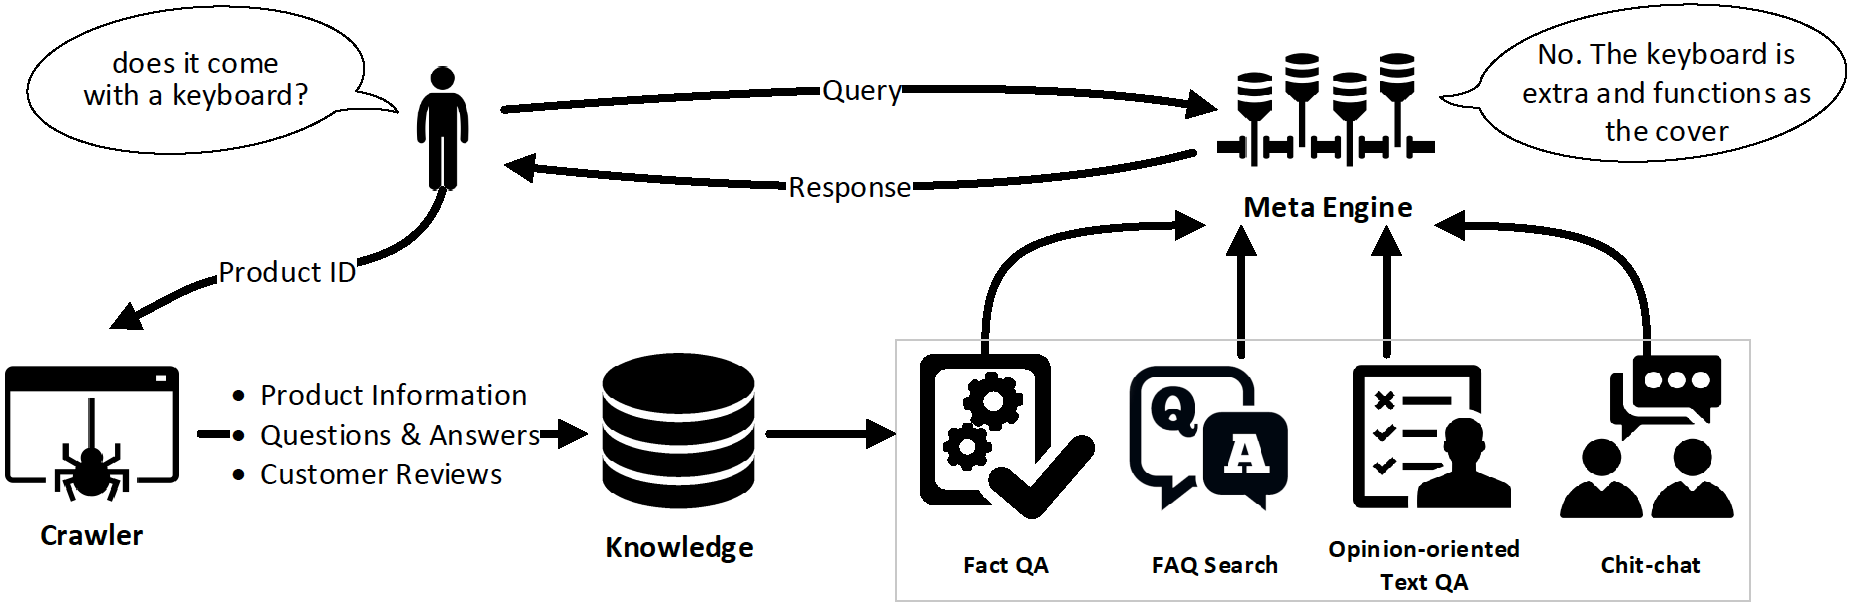
\includegraphics[scale=0.45]{chapter2/img/superagent.png}
        \end{center}
        \caption{Kiến trúc tổng quát của hệ thống SuperAgent}
        \label{fig:superagent}
    \end{figure}
\end{center}

Hình \ref{fig:superagent} mô tả tổng quan hệ thống của SuperAgent. Như hình cho thấy, khi trang sản phẩm được truy cập lần đầu tiên, SuperAgent thu thập các dữ liệu thông tin sản phẩm (PI), bộ câu hỏi và trả lời (QA) và phản hồi của khách hàng (CR) từ trang web. Ưu điểm của mẫu thiết kế này là họ không cần triển khai trình thu thập thông tin cho các trang web. Thay vào đó, khi người dùng truy cập trang, SuperAgent sẽ được thông báo vì có tiện ích bổ sung được liên kết với mỗi trang web. Do đó, SuperAgent mang lại rất ít lượt tải web bổ sung cho các trang web đã được lưu trữ. Bên cạnh đó, kiến trúc này giúp cho việc cập nhật dữ liệu rất dễ thực hiện, trong đó các trang được truy cập thường xuyên sẽ được cập nhật thường xuyên và ngược lại. Với một truy vấn đầu vào từ khách hàng, các công cụ khác nhau sẽ được xử lý song song. Nếu một trong ba câu trả lời từ ba công cụ đầu tiên có độ tin cậy cao, thì chatbot sẽ trả về câu trả lời từ phản hồi. Nếu không, công cụ trò chuyện sẽ tạo ra một câu trả lời từ các nhóm câu trả lời được phép xác định trước.

\begin{center}
    \begin{figure}[ht!]
        \begin{center}
         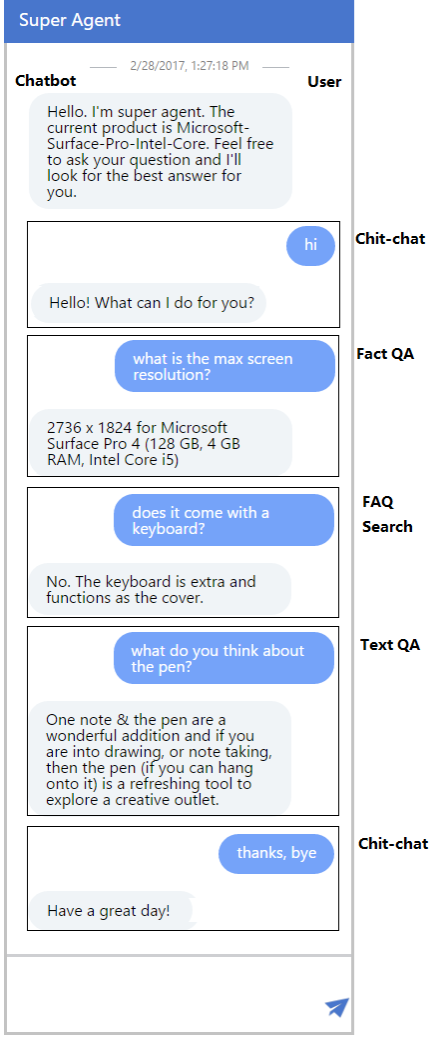
\includegraphics[scale=0.9]{chapter2/img/superagentdialog.png}
        \end{center}
        \caption{Một mẫu hội thoại của SuperAgent}
        \label{fig:superagentdialog}
    \end{figure}
\end{center}

Hình \ref{fig:superagentdialog} cho thấy một tình huống điển hình khi một khách hàng yêu cầu SuperAgent giúp đỡ. Khi khách hàng mở cửa sổ trò chuyện trong trình duyệt web, SuperAgent đầu tiên sẽ phát hiện sản phẩm nào đang được truy cập. Sau đó, SuperAgent tự giới thiệu và xác nhận rằng khách hàng đang ghé thăm sản phẩm. Khách hàng có thể chào hỏi SuperAgent hoặc hỏi các câu hỏi cụ thể. Như hình \ref{fig:superagentdialog} cho thấy, SuperAgent có thể trả lời các câu hỏi sự thật (Fact QA) bằng cách sử dụng thông tin sản phẩm trong trang, thực hiện tìm kiếm câu hỏi thường gặp (FAQ Search) từ các cặp QA của khách hàng, lấy câu trả lời QA từ đánh giá của khách hàng và cuối cùng là chào hỏi khách hàng bằng cách sử dụng công cụ trò chuyện chit-chat. Các hộp thoại được điều phối bởi công cụ meta để các truy vấn khác nhau chuyển đến các công cụ tương ứng. Vì các trang web thương mại điện tử được cập nhật thường xuyên và nội dung mới do người dùng tạo liên tục xuất hiện, SuperAgent cũng cập nhật dữ liệu và mô hình định kỳ theo tần suất truy cập của khách hàng.

\subsection{Bài báo về Chatbot hỗ trợ sân bay}
Đây là bài báo có tên \textit{Design and implementation of an airport chatbot} \cite{airport}. Trong bài báo này, họ mô tả động lực và quá trình phát triển của một Chatbot nhằm cung cấp thông tin và hỗ trợ cho khách du lịch trực tiếp bên trong nhà ga Sân bay Venice hoặc bằng các giao diện gián tiếp, chẳng hạn như ứng dụng di động hoặc trang web.

Để phát triển Chatbot, họ quyết định dựa trên một nền tảng được cung cấp bởi một công ty công nghệ lớn: Microsoft Azure Bot Service. Tất cả các dịch vụ cloud và dịch vụ máy chủ cho trang web và quản lý email đều đã được Microsoft quản lý. Họ sử dụng bộ xử lý ngôn ngữ tự nhiên để hiểu loại (ý định) và các tham số (thực thể) của câu hỏi mà người dùng có thể hỏi, bất kể nó được hỏi như thế nào. Ví dụ, trong Chatbot của họ, câu "what is the weather like in Venice?" (Thời tiết ở Venice như thế nào?) được chuyển thành một đối tượng như ví dụ \ref{exam:airport}, có thể được thao tác bởi Chatbot.

\renewcommand{\lstlistingname}{Ví dụ}
\begin{lstlisting}[caption={Biểu diễn của một câu hỏi},label={exam:airport},language=code_en,firstnumber=1]
{
    intent : "weather",
    parameters : {
        address : {
            city : "Venice"
        },
        date-time : "2019-01-20T12:00:00+02:00"
    }
}
\end{lstlisting}

Hệ thống họ phát triển có các chức năng sau:

\begin{itemize}
    \item Câu hỏi thường gặp (FAQ).
    \item Các câu hỏi chung về sân bay do tổng đài thu thập.
    \item Thông tin chuyến bay.
    \item Thông tin giao thông địa phương đến và đi từ sân bay (kế hoạch chuyến đi).
    \item Vị trí của các cửa hàng, hoạt động hoặc cổng bên trong sân bay.
    \item Thông tin về bãi đậu xe.
    \item Tìm hành lý thất lạc.
    \item Tìm đồ bị mất.
\end{itemize}

Sơ đồ chung của Chatbot được thể hiện trong hình \ref{fig:airportarch}. LUIS là dịch vụ xử lý như NLP. Nó có giao diện web cho phép tạo ra các ý định và thực thể nhưng không cung cấp phản hồi trực tiếp. Tích hợp LUIS cho phép bot hiểu ngôn ngữ tự nhiên, phát hiện lỗi chính tả, sử dụng nhận dạng giọng nói và nhận ra mục đích của người dùng. QnA Maker là một dịch vụ API dựa trên đám mây tạo ra một lớp câu hỏi và câu trả lời tương tự như một cuộc trò chuyện dữ liệu. Các câu hỏi và câu trả lời được nhập từ nội dung bán cấu trúc (semi-structure), chẳng hạn như tài liệu thường gặp, các đường dẫn và hướng dẫn sử dụng sản phẩm. Chatbot phải giao tiếp với các dịch vụ cơ sở dữ liệu và API của sân bay để trả lời các câu hỏi cụ thể liên quan đến sân bay.

Các câu hỏi của người dùng được quản lý và phân tích bởi bộ điều phối (dispatcher) để quyết định xem câu hỏi có yêu cầu phản hồi linh động hay không, nếu có nó phải được gửi đến LUIS, hoặc câu hỏi tĩnh được gửi đến bộ tạo câu hỏi và trả lời (QnA). Quyền truy cập vào cơ sở hạ tầng sân bay nội bộ và các lệnh gọi API bên ngoài được thực hiện trực tiếp bởi dịch vụ bot Azure.

\begin{center}
    \begin{figure}[ht!]
        \begin{center}
         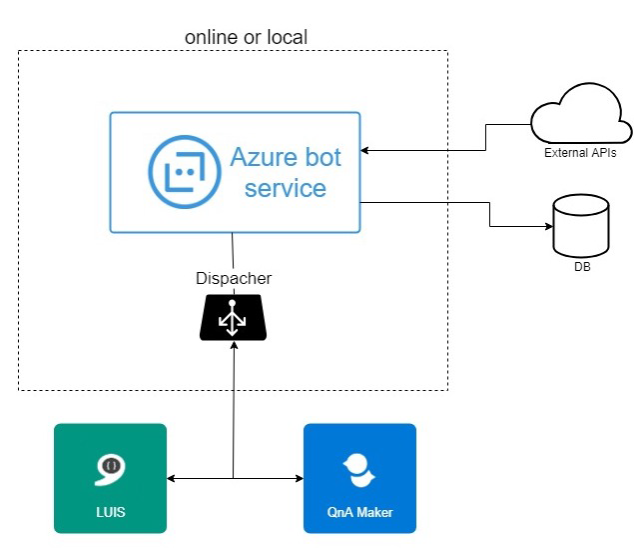
\includegraphics[scale=1]{chapter2/img/airportarch.png}
        \end{center}
        \caption{Sơ đồ tổng quát của Chatbot sân bay}
        \label{fig:airportarch}
    \end{figure}
\end{center}

\subsection{Bài báo về Chatbot hỗ trợ dịch vụ cung ứng}
Đây là bài báo có tên \textit{E-commerce Distributed Chatbot System} \cite{commerce}. Trong bài báo này, họ trình bày một hệ thống Chatbot phân tán cho chuỗi cung ứng. Hệ thống của họ bao gồm một số dịch vụ: dịch vụ trò chuyện, dịch vụ bot, dịch vụ xử lý ngôn ngữ tự nhiên và dịch vụ chuỗi cung ứng. Nó sử dụng giao tiếp WebSocket giữa giao diện người dùng và bot, phân tích truy vấn của người dùng và cung cấp thông tin về các đơn đặt hàng và nguồn cung cấp đã được truy vấn.

Kiến trúc hệ thống của Chatbot phân tán cho chuỗi cung ứng được đề xuất trong bài báo như trên hình \ref{fig:commerce}.

\begin{center}
    \begin{figure}[ht!]
        \begin{center}
         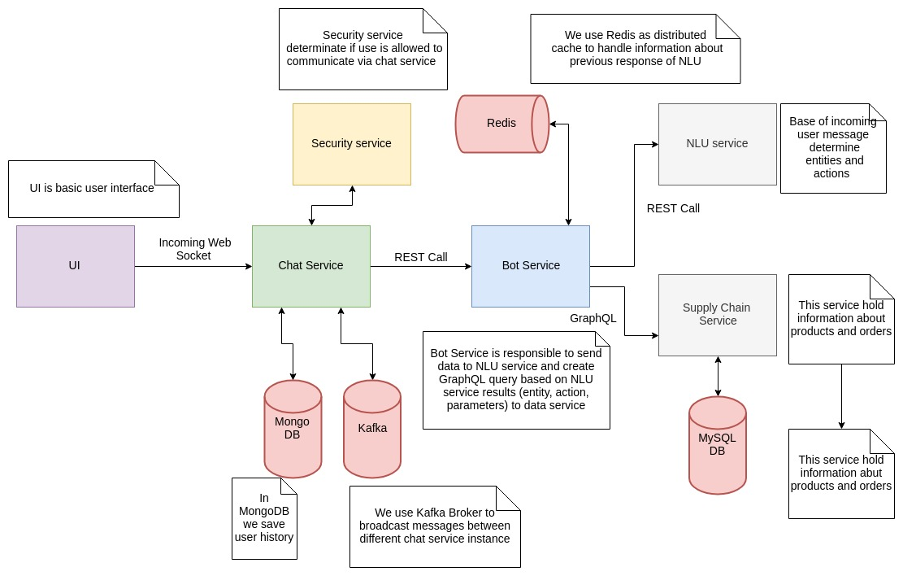
\includegraphics[scale=0.98]{chapter2/img/commerce.png}
        \end{center}
        \caption{Kiến trúc hệ thống Chatbot phân tán}
        \label{fig:commerce}
    \end{figure}
\end{center}

Hệ thống bao gồm năm dịch vụ con:
\begin{itemize}
    \item Dịch vụ trò chuyện (Chat Service): chịu trách nhiệm về giao tiếp WebSocket giữa giao diện người dùng và bot.
    \item Dịch vụ bot (Bot Service): phân tích thông điệp của người dùng, xây dựng yêu cầu truy xuất thông tin cần thiết và cung cấp cho người dùng một cách dễ hiểu.
    \item Dịch vụ hiểu ngôn ngữ tự nhiên (NLU Service): phân tích thông điệp của người dùng, trích xuất thông tin về ý định của người dùng và các đối tượng làm phong phú thêm thông tin về ý định đó.
    \item Dịch vụ chuỗi cung ứng (Supply Chain Service): chứa thông tin về đơn đặt hàng và nguồn cung cấp cho người dùng.
    \item Dịch vụ an ninh (Security Service): chịu trách nhiệm về bảo mật thông tin liên lạc qua dịch vụ trò chuyện.
\end{itemize}

Sơ đồ triển khai của hệ thống Chatbot phân tán cho chuỗi cung ứng dựa trên kiến trúc đề xuất được hiển thị trên hình \ref{fig:commercediagram}. Hệ thống được triển khai dưới dạng có tám bộ chứa docker.

\begin{center}
    \begin{figure}[ht!]
        \begin{center}
         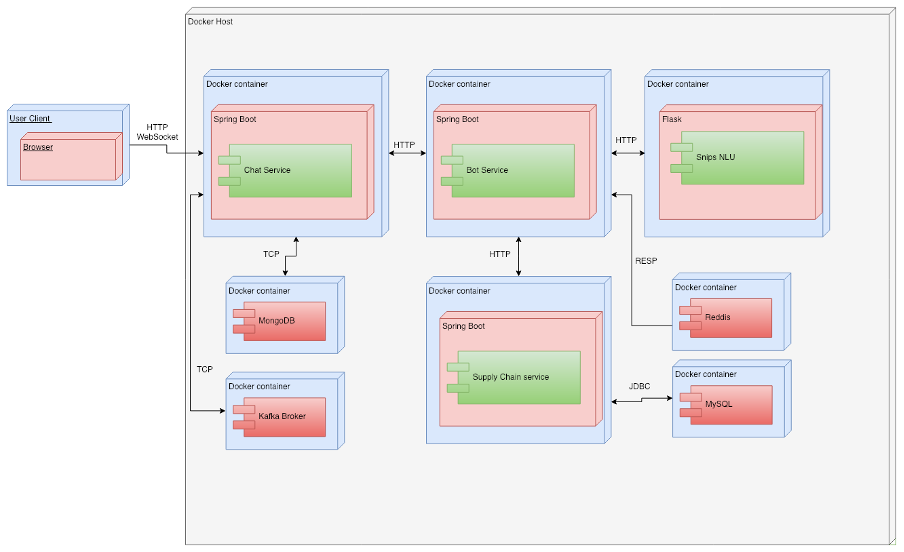
\includegraphics[scale=0.97]{chapter2/img/commerce_diagram.png}
        \end{center}
        \caption{Sơ đồ triển khai của hệ thống Chatbot phân tán}
        \label{fig:commercediagram}
    \end{figure}
\end{center}

Đánh giá thử nghiệm của họ đối với hệ thống Chatbot phân tán cho chuỗi cung ứng được dựa trên hai nhóm mẫu thử nghiệm: mẫu thử nghiệm tuân theo mẫu dữ liệu đào tạo và mẫu thử nghiệm sử dụng nhiều từ đồng nghĩa trong truy vấn của người dùng dựa trên ngôn ngữ tự nhiên.

Kết quả thử nghiệm của họ cho thấy khả năng nhận dạng đúng trong 90\% các câu người dùng thử nghiệm mẫu và tỷ lệ nhận dạng 65\% đối với các truy vấn của người dùng với các từ đồng nghĩa của các câu đó.

Chất lượng nhận dạng dịch vụ của NLU được tăng thêm lên 83\% đối với các truy vấn của người dùng khác với các mẫu tham chiếu, bằng cách đào tạo bổ sung hệ thống NLU với dữ liệu thử nghiệm không được giải quyết đúng cách.

Ngoài ra, họ còn đánh giá hiệu suất của nó bằng cách sử dụng thử nghiệm áp lực (stress test) thông qua Gatling. Kết quả thử nghiệm cho thấy rằng hệ thống có thể xử lý tới 10000 phiên người dùng mà không cần mở rộng bất kỳ máy chủ nào trong 60 phút. Độ trễ chính của hệ thống đến từ việc không thể triển khai nhiều kết nối WebSocket cùng một lúc.

\section{Các công trình nghiên cứu liên quan đến Chatbot sử dụng mô hình học tăng cường}
\subsection{Bài báo về Chatbot sử dụng hành động phân cụm và phần thưởng}
Đây là bài báo có tên \textit{Deep Reinforcement Learning for Chatbots Using Clustered Actions and Human-Likeness Rewards} \cite{clustered}. Trong bài báo này, sử dụng các hành động phân cụm thay vì lượng lớn các hành động và một bộ khen thưởng đơn giản dựa trên cách cho điểm giống con người thu được từ dữ liệu hội thoại giữa con người với con người.

Họ huấn luyện các tác nhân học tăng cường sâu (DRL) bằng cách sử dụng dữ liệu trò chuyện trong văn bản thô - mà không có bất kỳ chú thích thủ công nào.

Kịch bản học tập của họ như sau:

\begin{itemize}
    \item Lấy một tập dữ liệu về các cuộc hội thoại giữa con người với con người ở dạng văn bản thô, tác nhân sẽ đóng vai trò của một trong hai người trong cuộc hội thoại, để học cách chọn những câu giống người khi tiếp xúc với cả những câu giống người và không giống người.
    \item Các tương tác của môi trường-tác nhân bao gồm cả các tương tác dữ liệu-tác nhân - không có trình mô phỏng người dùng như trong các hệ thống hội thoại hướng tác vụ.
    \item Trong mỗi lượt hội thoại, tác nhân quan sát trạng thái của môi trường thông qua mạng nơ-ron học sâu. Mạng này nó mô hình hóa một biểu diễn của tất cả các câu được nêu ra trong cuộc hội thoại cùng với một tập hợp các câu trả lời của ứng viên hoặc hành động của tác nhân (các hành động được phân cụm theo phương pháp của họ).
    \item Sau đó tác nhân chọn một hành động, biểu diễn dựa trên mức từ của hành động được gửi đến môi trường.
    \item Tác nhân nhận được lịch sử hội thoại đã được cập nhật và phần thưởng cho hành động đó, cho đến khi đáp ứng điều kiện chấm dứt.
\end{itemize}

Quá trình này, được minh họa trong hình \ref{fig:clusterarch} — được thực hiện lặp đi lặp lại cho đến khi kết thúc một cuộc hội thoại cho nhiều cuộc hội thoại nếu cần, tức là cho đến khi không có cải thiện nào nữa về hiệu suất của tác nhân.

\begin{center}
    \begin{figure}[ht!]
        \begin{center}
         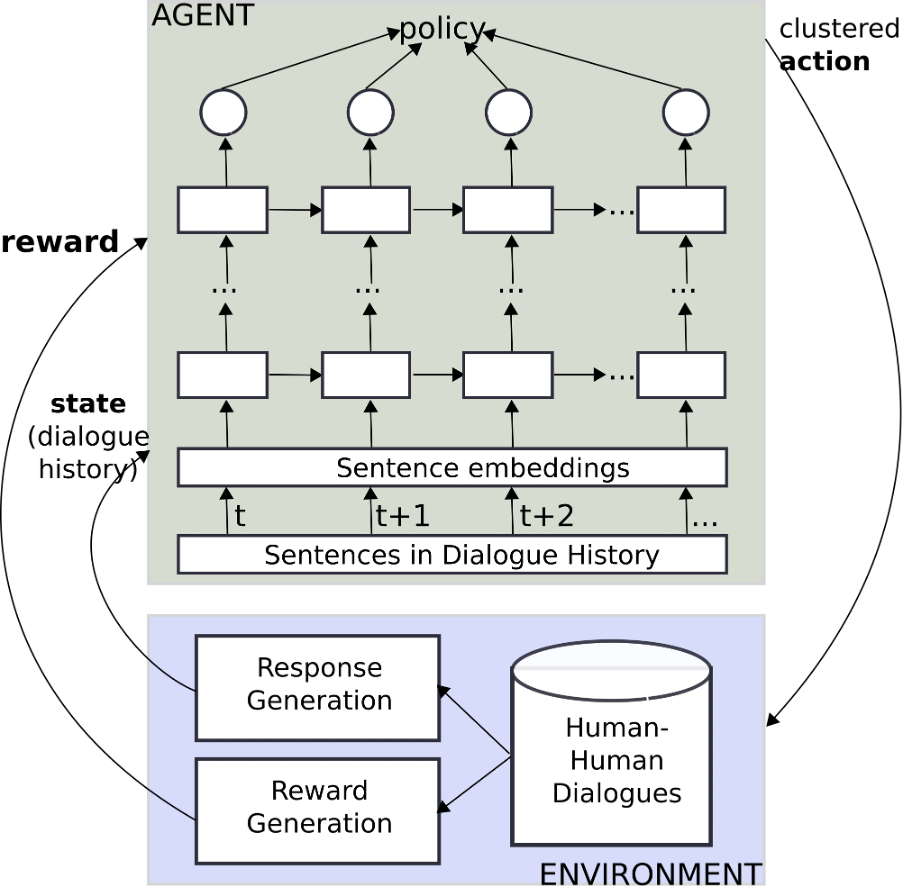
\includegraphics[scale=0.9]{chapter2/img/clusterarch.png}
        \end{center}
        \caption{Kiến trúc hệ thống Chatbot DRL}
        \label{fig:clusterarch}
    \end{figure}
\end{center}

Một số đóng góp của bài báo này như sau.

\begin{itemize}
    \item Họ đề xuất huấn luyện các Chatbot bằng cách sử dụng phương pháp học tăng cường dựa trên giá trị, bằng cách sử dụng không gian hành động bắt nguồn từ phân cụm không giám sát, trong đó mỗi cụm hành động là đại diện của một loại ý nghĩa (lời chào, câu hỏi xung quanh một chủ đề, phát biểu xung quanh một chủ đề, v.v.).
    \item Họ đề xuất một chức năng phần thưởng đơn giản nhưng đầy hứa hẹn. Nó dựa trên các cuộc hội thoại giữa con người với con người và các cuộc hội thoại nhiễu để học cách đánh giá các cuộc hội thoại tốt và xấu.
\end{itemize}

\subsection{Bài báo về hệ thống tạo đối thoại}
Đây là bài báo có tên \textit{Deep Reinforcement Learning for Dialogue Generation} \cite{generation}. Trong bài báo này, họ giới thiệu một phương pháp học tập tăng cường (RL), phương pháp này có thể tối ưu hóa phần thưởng dài hạn do các nhà phát triển hệ thống thiết kế. Mô hình của họ sử dụng kiến trúc bộ mã hóa giải mã (encoder-decoder) và mô phỏng cuộc trò chuyện giữa hai tác nhân ảo để khám phá không gian của các hành động có thể xảy ra trong khi học cách tối đa hóa phần thưởng mong đợi. Các tham số của bộ encoder-decoder RNN xác định chính sách (policy) trên một không gian hành động vô hạn bao gồm tất cả các cách phát biểu có thể có. Tác nhân tìm hiểu chính sách bằng cách tối ưu hóa phần thưởng dài hạn do nhà phát triển xác định từ các mô phỏng hội thoại đang diễn ra bằng cách sử dụng phương pháp gradient chính sách \cite{gradient}. Do đó, mô hình của họ tích hợp sức mạnh của hệ thống SEQ2SEQ để học các ý nghĩa ngữ nghĩa cấu thành của lời nói với các điểm mạnh của học tăng cường trong việc tối ưu hóa cho các mục tiêu dài hạn trong một cuộc trò chuyện.

Họ mô phỏng các cuộc trò chuyện giữa hai tác nhân ảo và để chúng thay phiên trò chuyện với nhau, như hình \ref{fig:generation}.

\begin{center}
    \begin{figure}[ht!]
        \begin{center}
         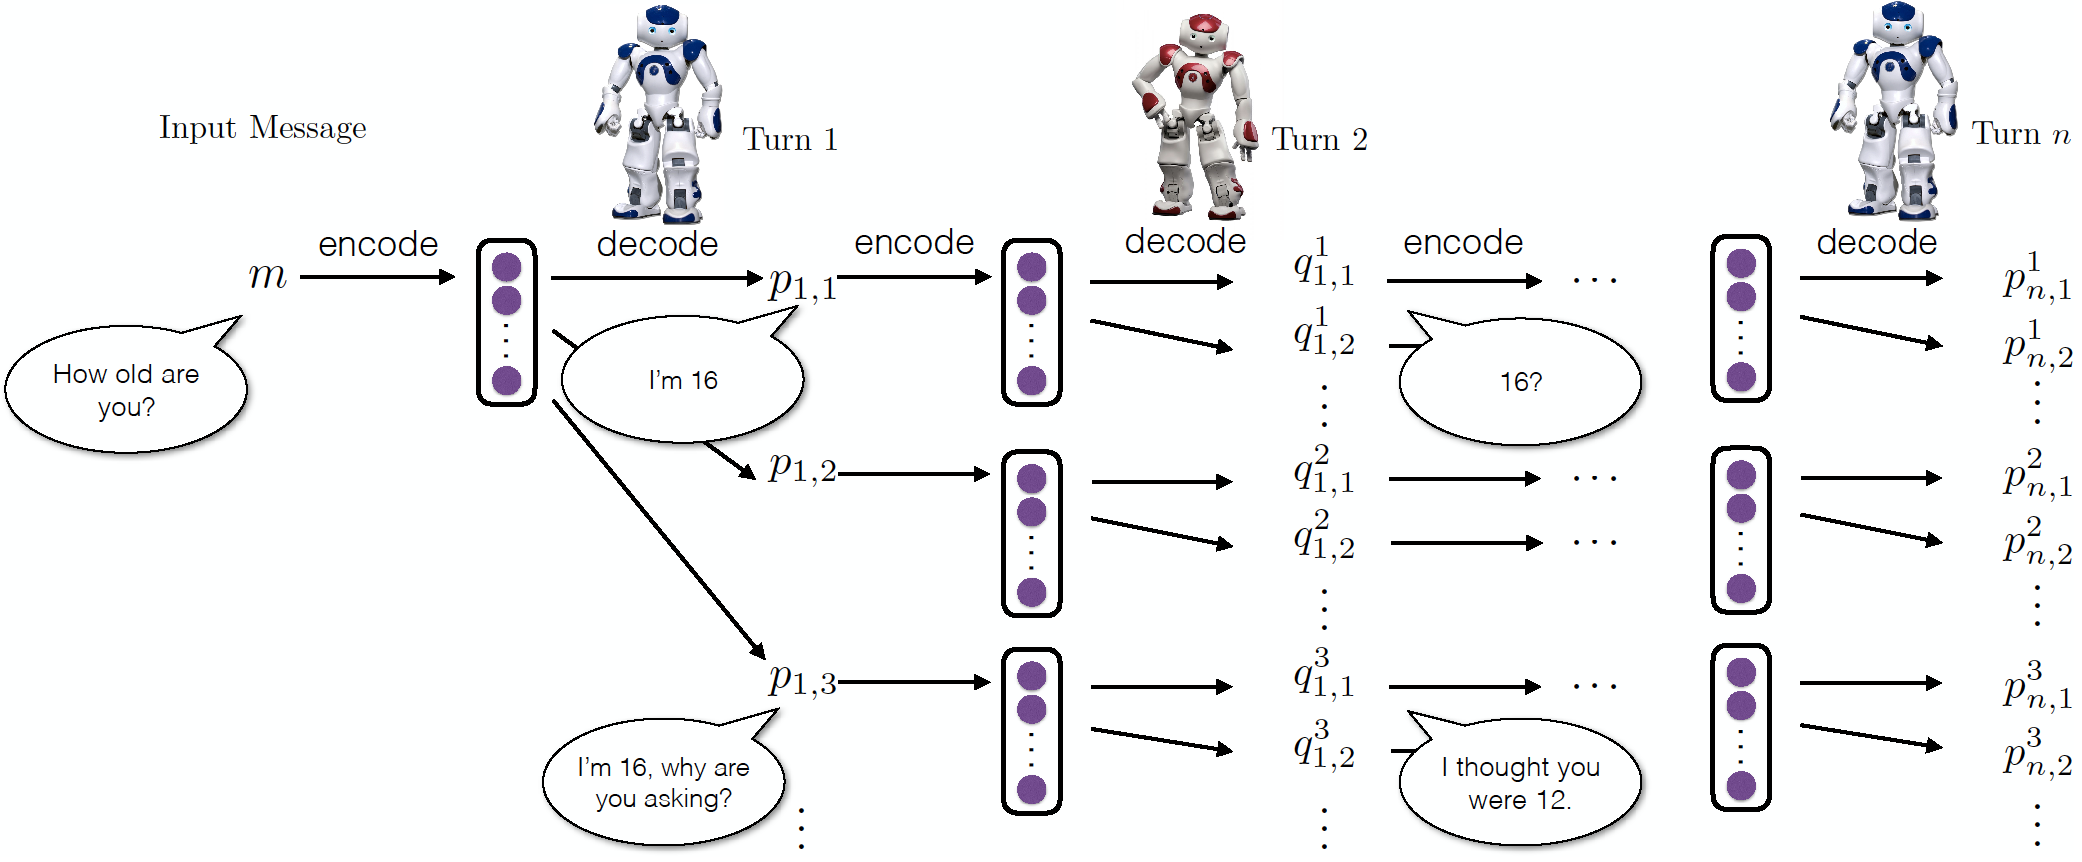
\includegraphics[scale=0.4]{chapter2/img/generation.png}
        \end{center}
        \caption{Mô phỏng đối thoại giữa hai tác nhân}
        \label{fig:generation}
    \end{figure}
\end{center}

Quá trình mô phỏng diễn ra như sau:

\begin{itemize}
    \item Ở bước đầu tiên, một thông báo từ tập huấn luyện được đưa đến tác nhân đầu tiên. Tác nhân mã hóa thông điệp đầu vào thành biểu diễn vec-tơ.
    \item Sau đó, bắt đầu giải mã để tạo ra đầu ra phản hồi.
    \item Kết hợp đầu ra ngay lập tức từ tác nhân đầu tiên với lịch sử đối thoại, tác nhân thứ hai cập nhật trạng thái bằng cách mã hóa lịch sử đối thoại thành một biểu diễn.
    \item Sau đó, sử dụng bộ giải mã RNN để tạo ra các phản hồi.
    \item Phản hồi được trả lại cho tác nhân đầu tiên và quá trình này được lặp đi lặp lại.
\end{itemize}

Kết quả thử nghiệm được lấy mẫu ở hình \ref{fig:generationdialog} chứng minh rằng cách tiếp cận của họ thúc đẩy một cuộc đối thoại bền vững hơn và quản lý để tạo ra nhiều phản hồi tương tác hơn so với các mô hình SEQ2SEQ tiêu chuẩn được đào tạo bằng cách sử dụng mục tiêu MLE.

\begin{center}
    \begin{figure}[ht!]
        \begin{center}
         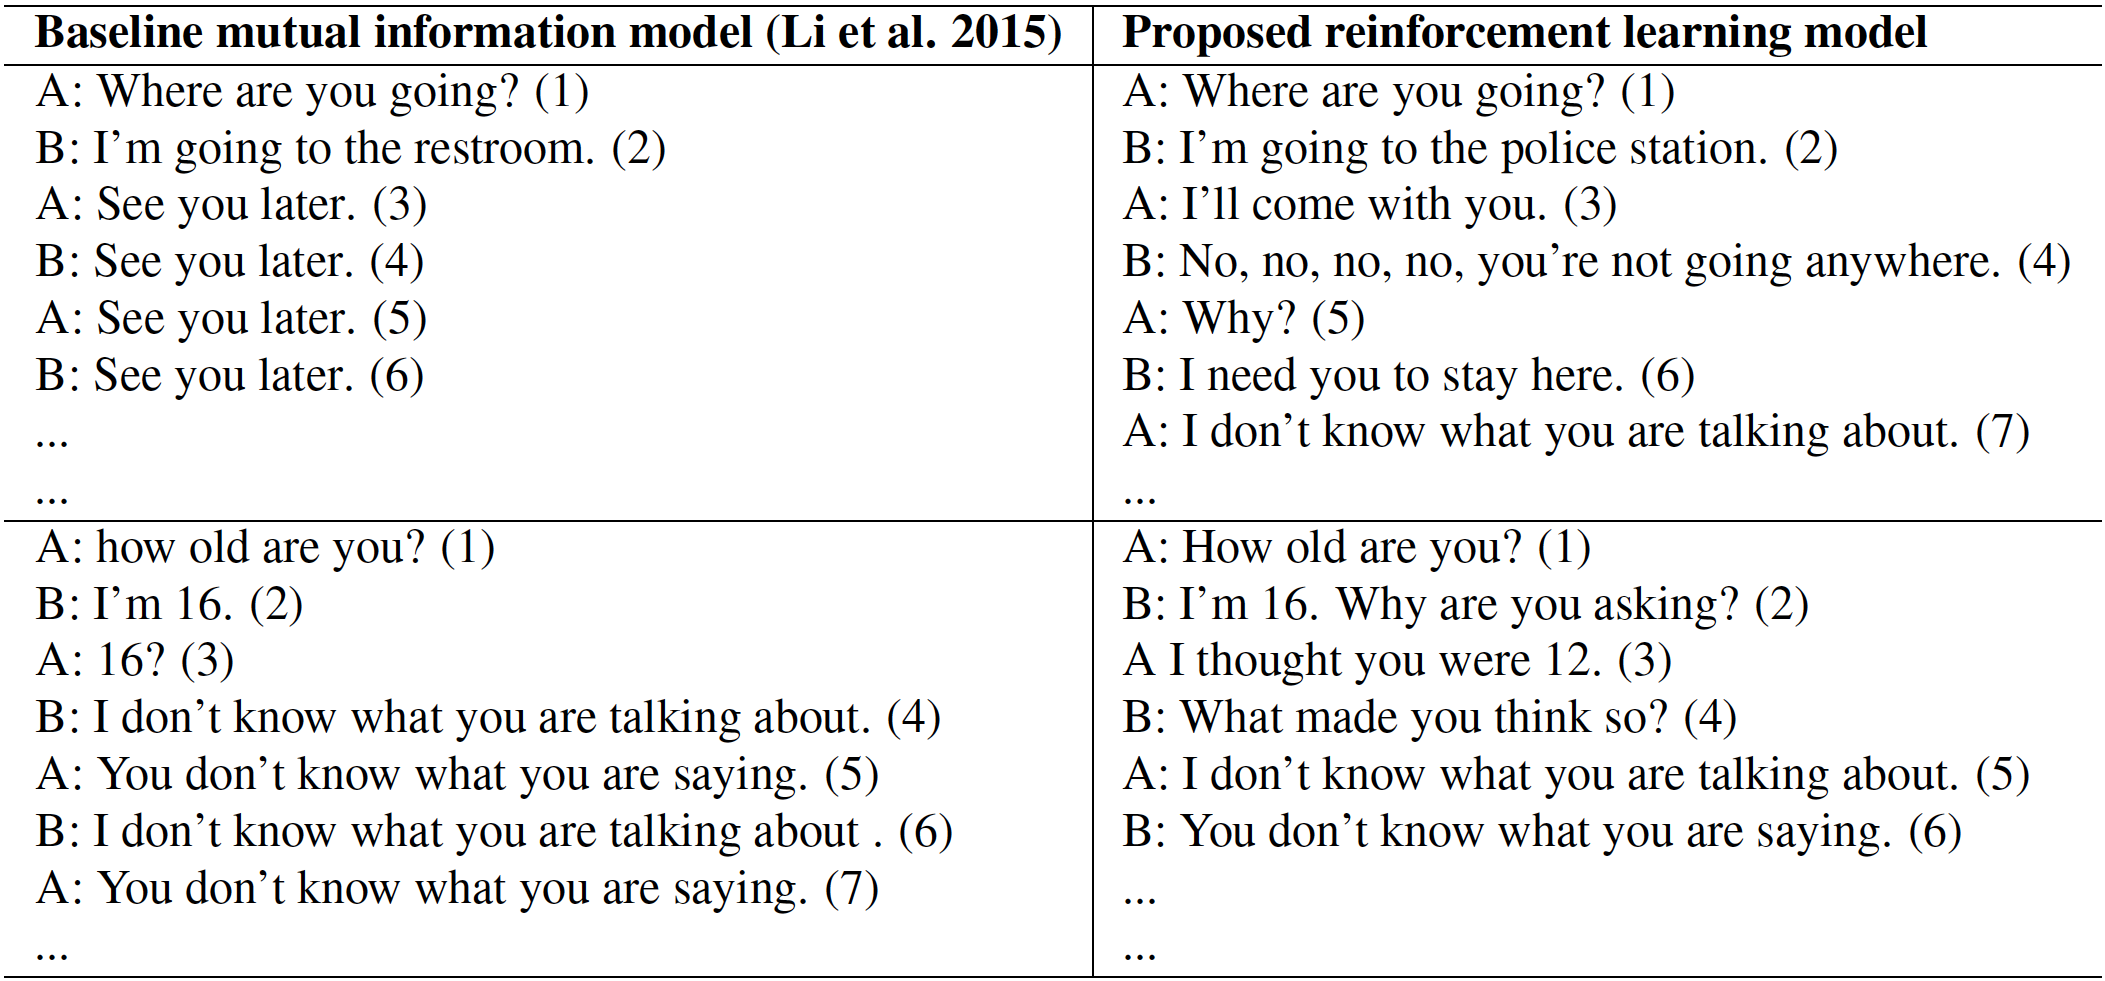
\includegraphics[scale=0.4]{chapter2/img/generationdialog.png}
        \end{center}
        \caption{Kết quả thử nghiệm của hai mô hình}
        \label{fig:generationdialog}
    \end{figure}
\end{center}

Cột bên trái: Mô phỏng đối thoại giữa hai tác nhân sử dụng bộ mã hóa-giải mã LSTM 4 lớp được đào tạo trên tập dữ liệu OpenSubtitles. Lượt đầu tiên (chỉ số 1) được nhập bởi các tác giả. Sau đó, hai tác nhân thay phiên nhau trò chuyện, lấy đầu vào cho lượt tạo trước của tác nhân kia. Cột Bên phải: Cuộc đối thoại được mô phỏng bằng cách sử dụng mô hình học tập tăng cường được đề xuất. Mô hình mới có nhiều cách nói hướng tới tương lai hơn (những câu hỏi như "Why are you asking?" và những lời đề nghị như "I'll come with you") giúp cuộc hội thoại diễn biến lâu hơn trước khi rơi vào hố đen (black holes).

\subsection{Bài báo về Chatbot FAQ}
Đây là bài báo có tên \textit{Self-improving Chatbots based on Reinforcement Learning} \cite{selfimproving}. Trong bài báo này, họ giới thiệu mô hình học tăng cường (RL) cho các Chatbot tự cải thiện, nhắm mục tiêu cụ thể đến các Chatbot dạng câu hỏi thường gặp (FAQ).

Mô hình này không nhằm mục đích xây dựng hệ thống hội thoại từ đầu mà nhằm tận dụng dữ liệu từ các cuộc trò chuyện của người dùng để cải thiện hiệu suất Chatbot. Cốt lõi của phương pháp tiếp cận của họ là mô hình điểm số, được đào tạo để tính điểm các câu trả lời của Chatbot dựa trên phản hồi của người dùng. Điểm số được dự đoán bởi mô hình này được sử dụng làm phần thưởng cho tác nhân. Việc học chính sách diễn ra ngoại tuyến, nhờ vào trình mô phỏng người dùng được cung cấp các câu thoại từ cơ sở dữ liệu FAQ. Học chính sách được triển khai bằng cách sử dụng tác nhân Deep Q-Network (DQN) với tính năng thăm dò tham lam (epsilon-greedy), được điều chỉnh để đưa vào một cách hiệu quả các câu trả lời dự phòng cho các câu hỏi ngoài phạm vi.

Kiến trúc mô hình được minh họa trong hình \ref{fig:selfimprovingarch}.

\begin{center}
    \begin{figure}[ht!]
        \begin{center}
         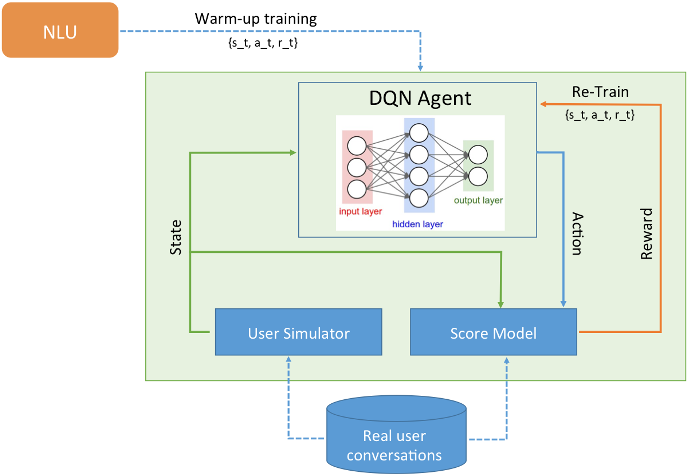
\includegraphics[scale=1]{chapter2/img/selfimproving_arch.png}
        \end{center}
        \caption{Kiến trúc của mô hình Chatbot FAQ}
        \label{fig:selfimprovingarch}
    \end{figure}
\end{center}

Các thành phần khác nhau của mô hình bao gồm:
\begin{itemize}
    \item Bộ hiểu ngôn ngữ tự nhiên (NLU), được sử dụng để huấn luyện tác nhân trong giai đoạn khởi động.
    \item Bộ mô phỏng người dùng (User Simulator), trích xuất ngẫu nhiên câu thoại của người dùng từ cơ sở dữ liệu về trải nghiệm người dùng.
    \item Mô hình điểm số (Score Model) được huấn luyện trên cuộc trò chuyện của người dùng với phản hồi và tác nhân dựa trên mạng Deep Q-Network (DQN).
\end{itemize}

Tác nhân DQN ban đầu được huấn luyện ngoại tuyến trong giai đoạn khởi động với NLU. Mô hình điểm số cũng được huấn luyện ngoại tuyến với dữ liệu từ các cuộc trò chuyện của người dùng thực. Trong vòng lặp học tăng cường, trạng thái người dùng (lời phát biểu của người dùng) được cung cấp bởi trình mô phỏng người dùng, hành động (phản hồi chatbot) được cung cấp bởi tác nhân DQN và phần thưởng được cung cấp bởi mô hình điểm. Mỗi tuple $(s_t, a_t, r_t)$ cung cấp bộ đệm phát lại trải nghiệm (experience replay), được sử dụng để huấn luyện lại DQN sau $n_{episodes}$ số lượt, là một tham số có thể điều chỉnh được.

Tiềm năng của phương pháp tiếp cận của họ được thể hiện trên một trường hợp nhỏ được trích xuất từ một Chatbot doanh nghiệp. Nó cho thấy sự gia tăng hiệu suất từ tỷ lệ thành công 50\% ban đầu lên 75\% trong 20-30 epoch huấn luyện.

\subsection{Chuỗi bài hướng dẫn huấn luyện Chatbot hướng mục tiêu sử dụng học tăng cường}
\label{subsec:training}
Đây là chuỗi bài hướng dẫn \cite{traininggochatbot} được thực hiện bởi một kênh nổi tiếng trên diễn đàn Medium - Towards Data Science. Điểm nổi bật của chuỗi bài này là tác giả đã xây dựng được một kiến trúc hệ thống học tăng cường (Reinforcement Learning) khá hoàn thiện, áp dụng cho bài toán tư vấn có mục tiêu cụ thể. Đặc biệt, có sử dụng hệ thống giả lập người dùng (User Simulator) với một số luật đơn giản để giúp hệ thống học tăng cường có thể học được nhanh hơn rất nhiều thay vì phải cần người thật tương tác. Những kiến thức đó được tác giả vận dụng từ một bài báo \cite{endtoend} của nhóm nghiên cứu đến từ phòng nghiên cứu của Microsoft, Hoa Kỳ. Cụ thể, kiến trúc mà tác giả đề cập tới bao gồm bốn phần chính là \textit{Agent} (tác nhân - đối tượng sẽ được huấn luyện để ra quyết định), \textit{Dialog State Tracker} (đối tượng quản lý trạng thái hội thoại), \textit{User Simulator} (đối tượng giả lập người dùng - mục đích giúp quá trình huấn luyện nhanh chóng hơn) và \textit{EMC - Error Model Controller} (mô phỏng lỗi - giúp tác nhân học hiệu quả hơn).

Bài toán mà tác giả nêu ra trong bài viết của mình là tư vấn chọn vé xem phim. Dữ liệu là các thông tin của xuất phim và được lưu dưới ở dạng các cặp khóa - giá trị như biểu diễn ở ví dụ \ref{exam:dbmovie}.

\renewcommand{\lstlistingname}{Ví dụ}
\begin{lstlisting}[caption={Dữ liệu thông tin của các xuất phim},label={exam:dbmovie},language=code_en,firstnumber=1]
0L: {'city': 'hamilton', 'theater': 'manville 12 plex', 'zip': '08835', 'critic_rating': 'good', 'genre': 'comedy', 'state': 'nj', 'starttime': '10:30am', 'date': 'tomorrow', 'moviename': 'zootopia'}
897L: {'city': 'seattle', 'theater': 'pacific place 11', 'moviename': 'how to be single', 'zip': '98101', 'critic_rating': 'top', 'date': 'tonight', 'state': 'washington', 'other': 'date', 'starttime': '9', 'theater_chain': 'amc', 'genre': 'romance'}
\end{lstlisting}

Các khóa như "0L" hay "897L" là khóa định danh của từng xuất phim có kiểu dữ liệu số nguyên và giá trị của nó cũng ở dạng các cặp khóa - giá trị (một kiểu \textit{dictionary} trong \textit{python}) có chứa các thông tin (city, theater, zip, v.v.). Các xuất phim không có số lượng các thông tin giống nhau và các giá trị của thông tin cũng khác nhau.

Ngoài ra, họ còn có một loại dữ liệu nữa là từ điển (database dictionary) chứa tất cả các giá trị có thể có của từng thông tin với mục đích là dùng cho bộ \textit{EMC} để tạo ra lỗi, cấu trúc được biểu diễn như ở ví dụ \ref{exam:dictmovie}.

\renewcommand{\lstlistingname}{Ví dụ}
\begin{lstlisting}[caption={Từ điển của các thông tin xuất phim},label={exam:dictmovie},language=code_en,firstnumber=1]
'city': ['hamilton', 'manville', 'bridgewater', 'seattle', 'bellevue', 'birmingham', 'san francisco', 'portland', ...]
'theater': ['manville 12 plex', 'amc dine-in theatres bridgewater 7', 'bridgewater', 'every single theatre', ...]
\end{lstlisting}

Loại dữ liệu thứ ba được tác giả đề cập tới là danh sách mục tiêu người dùng (user goal) chứa tất cả mục tiêu có thể có của người dùng khi họ bắt đầu một cuộc hội thoại với Chatbot. Dữ liệu này sẽ được \textit{User Simulator} sử dụng trong quá trình huấn luyện \textit{agent}, cấu trúc bao gồm:

\begin{itemize}
    \item \textit{inform slots}: các thông tin người dùng sẽ cung cấp cho \textit{agent}.
    \item \textit{request slots}: các thông tin người dùng yêu cầu nhận được từ \textit{agent}.
\end{itemize}

\textit{Inform slots} và \textit{request slots} có thể có giá trị hoặc rỗng. Cấu trúc được biểu diễn như ở ví dụ \ref{exam:goalmovie}.

\renewcommand{\lstlistingname}{Ví dụ}
\begin{lstlisting}[caption={Mục tiêu người dùng của hệ thống tư vấn chọn vé xem phim},label={exam:goalmovie},language=code_en,firstnumber=1]
{'request_slots': {'date': 'UNK', 'theater': 'UNK'}, 'inform_slots': {'numberofpeople': '4', 'moviename': 'zootopia', 'starttime': 'matinee'}}
{'request_slots': {'theater': 'UNK'}, 'inform_slots': {'city': 'la', 'numberofpeople': '2', 'distanceconstraints': 'downtown', 'video_format': '3d', 'starttime': '7pm', 'date': 'tomorrow', 'moviename': 'creed'}}
\end{lstlisting}

Một khái niệm được đề cập xuyên suốt gọi là \textit{action}. \textit{Action} mô tả một hành động và dựa trên nó, ta có thể sinh ra câu phản hồi. Hệ thống không làm việc trực tiếp với câu dưới dạng ngôn ngữ tự nhiên mà thông qua \textit{action}. Một \textit{action} sẽ có \textit{inform slots} và \textit{request slots} giống \textit{user goal} như đã nêu ở trên đồng thời có thêm \textit{intent} - ý định của người dùng hoặc của \textit{agent} ứng với mỗi câu thoại diễn ra trong hội thoại. Với bài toán tư vấn vé xem phim, tác giả đã định nghĩa các loại \textit{intent} như:

\begin{itemize}
    \item \textbf{Inform:} cung cấp những điều kiện ràng buộc, thông tin được trình bày trong \textit{inform slots}.
    \item \textbf{Request:} yêu cầu giá trị cho các thông tin được trình bày trong \textit{request slots}.
    \item \textbf{Thanks:} chỉ thực hiện bởi người dùng, thể hiện cho \textit{agent} biết rằng nó đã làm gì đó tốt hoặc người dùng đã sẵn sàng kết thúc cuộc hội thoại.
    \item \textbf{Match Found:} chỉ thực hiện bởi \textit{agent}, thông báo cho người dùng biết rằng nó đã tìm được thông tin thỏa mãn các điều kiện ràng buộc của người dùng.
    \item \textbf{Reject:} chỉ thực hiện bởi người dùng, báo cho \textit{agent} biết rằng thông tin nó vừa thông báo không thỏa mãn yêu cầu ràng buộc của người dùng.
    \item \textbf{Done:} \textit{agent} sử dụng để báo rằng nó đã hoàn thành mục tiêu hội thoại. Người dùng sử dụng \textit{intent} này để kết thúc hội thoại.
\end{itemize}

Khái niệm đi kèm với \textit{action} là \textit{state} - trạng thái của cuộc hội thoại. Nó đóng vai trò là đầu vào cho \textit{agent} để chọn ra một \textit{action} phù hợp nhất. \textit{State} thực chất là một ma trận mã hóa toàn bộ lịch sử hội thoại từ lúc bắt đầu cho tới thời điểm hiện tại.

Hình \ref{fig:trainrefer} mô tả một vòng huấn luyện của hệ thống này sẽ được diễn ra. Cụ thể:

\begin{center}
    \begin{figure}[ht!]
        \begin{center}
         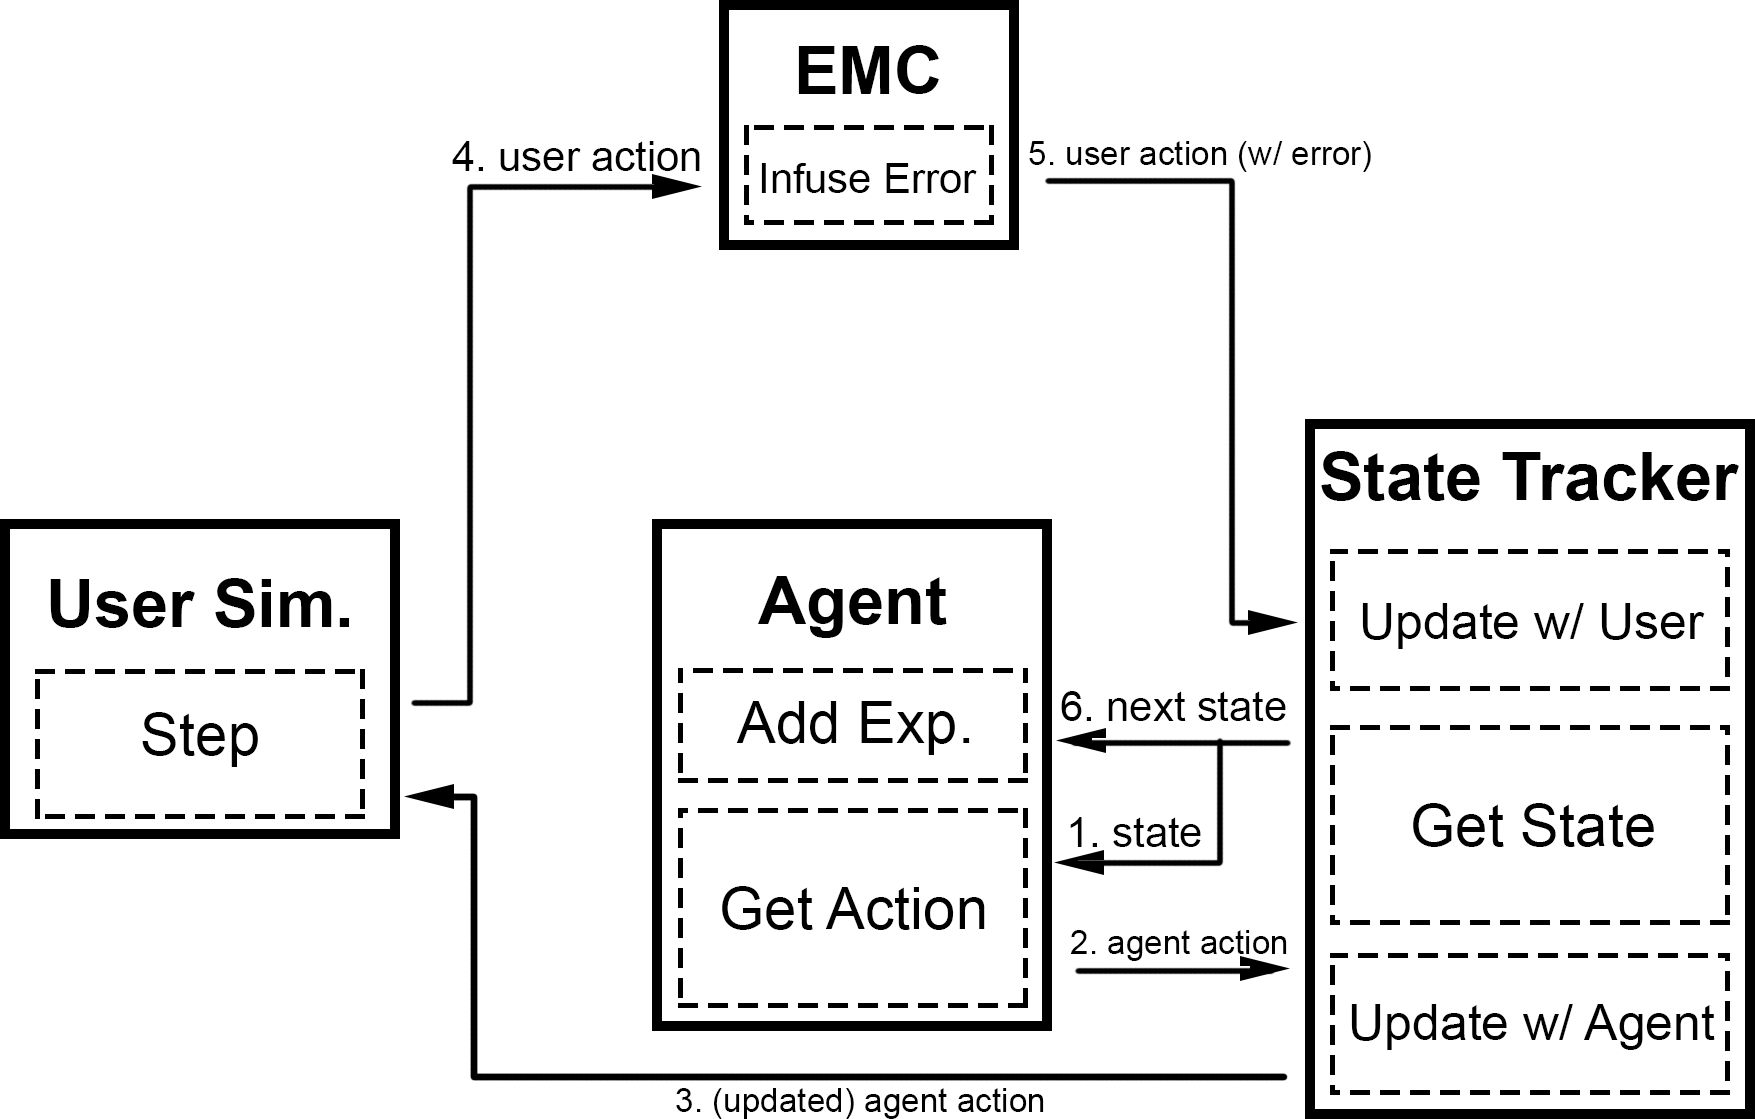
\includegraphics[scale=0.23]{chapter2/img/train_refer.png}
        \end{center}
        \caption{Kiến trúc tổng quát của mô hình RL agent}
        \label{fig:trainrefer}
    \end{figure}
\end{center}

\begin{itemize}
    \item \textbf{Bước 1:} Lấy ra \textit{state} - trạng thái hiện tại từ \textit{State Tracker}, \textit{state} này có thể là \textit{state} khởi tạo nếu như vừa bắt đầu hội thoại hoặc là \textit{state} của toàn bộ cuộc hội thoại giữa người dùng và Chatbot. \textit{State} sau khi được lấy ra sẽ làm đầu vào (input) cho \textit{agent} ở bước tiếp theo.
    \item \textbf{Bước 2:} \textit{Agent} sau khi nhận được input từ bước trước sẽ sinh ra \textit{action} và gửi ngược về lại \textit{State Tracker}. \textit{Action} lúc này ở dạng thô, chưa kèm thông tin cụ thể. Nó sẽ được \textit{State Tracker} cập nhật thông tin sau khi thực hiện truy vấn lên cơ sở dữ liệu. Đồng thời \textit{State Tracker} cũng sẽ cập nhật lại trạng thái của hội thoại.
    \item \textbf{Bước 3:} \textit{Action} sau khi được cập nhật đầy đủ thông tin sẽ được gửi cho \textit{User Simulator}. \textit{User Simulator} sẽ dựa vào các luật đã được quy định trước để sinh ra \textit{action} (có cấu trúc tương tự \textit{action} của \textit{agent} ở bước trước), kèm theo \textit{reward} (điểm thưởng) và tín hiệu success (thành công) để giúp \textit{agent} có thể tự điều chỉnh hành vi để học.
    \item \textbf{Bước 4:} \textit{Action} của người dùng ở bước trước đó sẽ được đưa qua \textit{EMC}, mục đích là tạo ra các lỗi mà người dùng thật hay mắc phải, giúp \textit{agent} có hành vi chính xác và tự nhiên hơn khi chạy ở thực tế.
    \item \textbf{Bước 5:} \textit{Action} ở bước trước sẽ tiếp tục được gửi đi đến \textit{State Tracker} và được cập nhật thông tin cụ thể tương tự ở bước 2. Đồng thời \textit{State Tracker} cũng cập nhật trạng thái của nó.
    \item \textbf{Bước 6:} Trạng thái tiếp theo được lấy từ \textit{State Tracker} và quay lại giống bước 1.
\end{itemize}

\section{Kết luận}
Hiện nay, có rất nhiều nghiên cứu, công trình liên quan đến xây dựng một Chatbot tư vấn khách hàng trong nhiều lĩnh vực cũng như các nghiên cứu cụ thể liên quan đến mô hình sử dụng học tăng cường như đã trình bày ở một số công trình ở trên.

Trong đó, các công trình xây dựng Chatbot cho các dịch vụ tư vấn sử dụng các phương pháp đa dạng, từ đơn giản như sử dụng cấu trúc ngôn ngữ và so trùng cho đến áp dụng các bộ xử lý ngôn ngữ tự nhiên, huấn luyện mô hình hay để tiết kiệm nguồn lực và chi phí sử dụng các nền tảng sẵn có. Việc này cũng tùy thuộc vào lĩnh vực của Chatbot hoạt động.

Các hướng tiếp cận sử dụng mô hình học tăng cường cũng được áp dụng trên nhiều lĩnh vực khác nhau. Kết quả của những nghiên cứu trên cũng thể hiện được điểm mạnh của mô hình này. Các tác nhân có các phản hồi linh hoạt hơn, với cơ chế tự học cũng giúp nó không giới hạn khả năng. Lý giải tại sao giải thuật học tăng cường được áp dụng mạnh mẽ trong các hệ thống Chatbot. Vì vậy trong luận văn này cũng đã áp dụng phương pháp này. Cụ thể, đề tài tham khảo một kiến trúc huấn luyện mô hình học tăng cường hướng mục tiêu được trình bày ở mục \ref{subsec:training}.
